\documentclass[12pt,a4paper,final,twoside]{article}
\usepackage[utf8]{inputenc}
\usepackage[catalan]{babel}

\usepackage{hyperref}
\usepackage{url}

\usepackage{setspace}
\onehalfspacing

\usepackage{amsmath}
\usepackage{amssymb}
\usepackage{multirow}
\usepackage{graphicx}
\usepackage{caption}
\usepackage{subcaption}
\usepackage{framed}

\usepackage[ampersand]{easylist}

\usepackage{array}
\usepackage{multirow}
\usepackage{tabulary}

\usepackage{float}

\usepackage[left=2.5cm,right=2.5cm,top=2.5cm,bottom=2.5cm]{geometry}

\usepackage{appendix}
\renewcommand{\appendixname}{Annexos}
\renewcommand{\appendixtocname}{Annexos}
\renewcommand{\appendixpagename}{Annexos}


%\usepackage[nomain,acronym,toc]{glossaries}
% nomain, if you define glossaries in a file, and you use 
%\include{./Glossari/glossari}
%\makeglossaries

%Pendent el fer el glossari

\usepackage{imakeidx}
\makeindex

\usepackage{wrapfig}

%\usepackage{makeidx}
%\makeindex

\usepackage{fancyhdr}
\pagestyle{fancy}
\fancyhead{}
\fancyhead[RO,LE]{\thepage}
\fancyhead[RE,LO]{Aibo}
\fancyfoot{}
\fancyfoot[RO,LE]{
\includegraphics[scale=0.3]{Imatges/etseib.jpg}}

\headheight = 15pt %Donava un warning sino

\textheight = 690pt %Col·locació de l'escut a distancia que quedi be
\footskip = 60pt

\usepackage[numbers]{natbib}
\bibliographystyle{plainnat} 
%Poso per ordre de apració (així) o per ordre d'autors (plainnat)?

\title{Aibo}
\author{Lluís Salord Quetglas\\
		\texttt{l.salord.quetglas@gmail.com}\\}
\date{\today}




\begin{document}
\maketitle
\thispagestyle{empty}
\begin{figure}[h!]
\centering
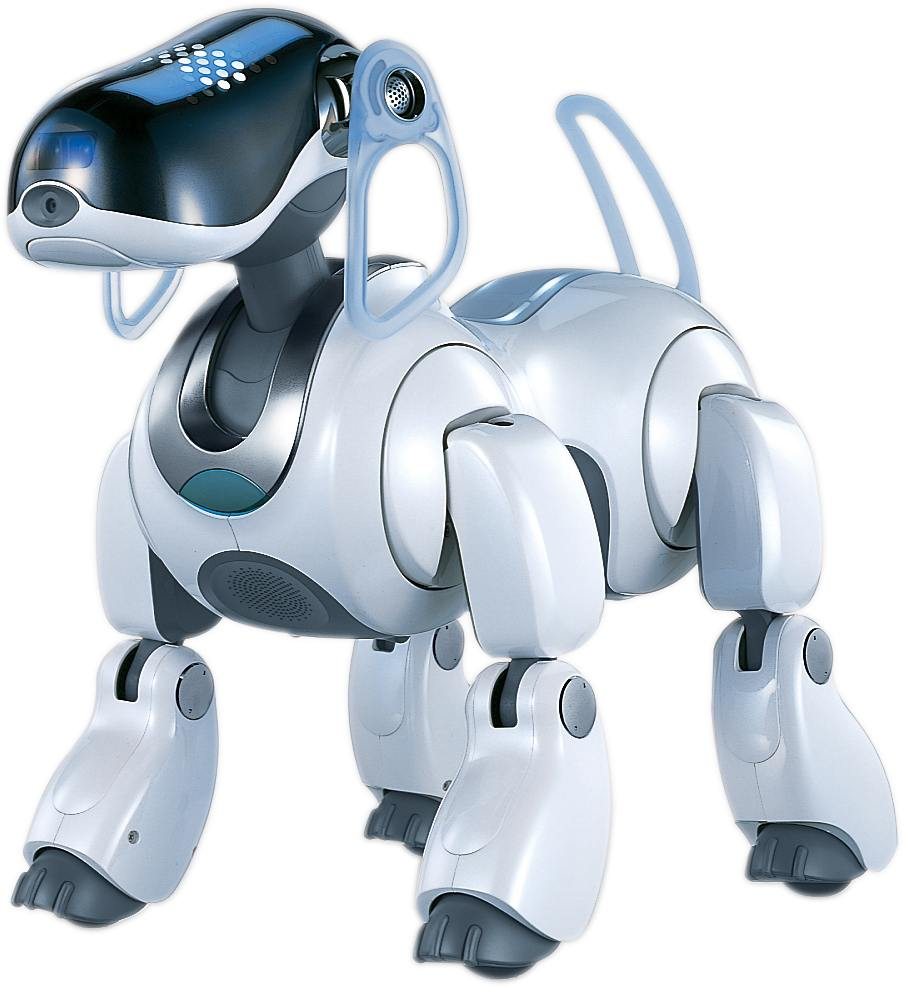
\includegraphics[scale=0.1]{Imatges/ERS7.jpg} 
\end{figure}

\newpage
\paragraph{}
\thispagestyle{empty}
\cleardoublepage

\setcounter{page}{1} %Començar en la pagina 1

\begin{abstract}
\addcontentsline{toc}{section}{Resum}
L'estabilitat del robots...
\end{abstract}

\renewcommand{\abstractname}{Resumen}
\begin{abstract}
\addcontentsline{toc}{section}{Resumen}
La estabilidad de los robots...
\end{abstract}

\renewcommand{\abstractname}{Abstract}
\begin{abstract}
\addcontentsline{toc}{section}{Abstract}
The estability of the robots...
\end{abstract}
\newpage
\cleardoublepage

\tableofcontents
\newpage
\listoffigures
\newpage
\listoftables
\newpage


%\printglossary
%\newpage

\label{Prefaci}
\section*{Prefaci}
\addcontentsline{toc}{section}{Prefaci}

\label{Motivacio}
\subsection*{Motivació}
\addcontentsline{toc}{subsection}{Motivació}

\paragraph{}Moltes persones que tenen devoció pel món de la robòtica els hi ha vingut des de ben joves, aquest no és el meu cas. A mi, el que m'agradava era la informàtica. Sent petit vaig aprendre de forma autodidacte a programar en \textit{C++} i crear un servidor propi. Fet que ajudà, en arribar a la UPC, a divertir-me amb assignatures relacionades amb programació, però em faltava veure reflectit el meu treball amb alguna utilitat física. No va ser fins que en Projecte II, vam controlar un mecanisme a través d'un microcontrolador \textit{Arduino}\footnote{\textit{Arduino} és la marca d'una família de microcontrolador}, amb programació basada en \textit{Wiring} \cite{Arduino}, llavors vaig veure clar cap on volia enfocar el meu futur, la robòtica.

\paragraph{}D'aquesta motivació que ha crescut poc a poc n'ha sorgit el perquè d'escollir aquest TFG. A més, a cada pas que he fet en el treball, com més he vist i entès la gran complexitat d'altres robots, com el \textit{Big Dog} del \textit{Boston Dinamics} o el \textit{NAO} de \textit{Aldebaran Robotics}\footnote{En l'estat de l'art es dona una breu explicació d'aquests i altres robots}, entre d'altres, més estímuls tenia per avançar i millorar.

\paragraph{}Ara bé, deixant de banda les pròpies ganes de treballar en robòtica, també he tingut en compte la preparació pel futur professional. Per això, en molts casos, a l'hora de fer alguna elecció, he intentat escollir la que fos més innovadora i útil el dia de demà. Aquest fet es veu tant en l'elecció dels llenguatges utilitzats com també en l'algorisme de resolució de la problemàtica de treball en qüestió. Per tant, queda palès que aquest treball té com a motivació la combinació d'entusiasme pel món de la robòtica i la millora d'un mateix per tal de poder arribar a un bon futur professional en aquest camp.

\label{Requeriments}
\subsection*{Requeriments previs}
\addcontentsline{toc}{subsection}{Requeriments previs}

\paragraph{}En el TFG aquí present, tot i que s'ha intentat donar una explicació a cada concepte que podria no haver-se entès, es necessari tenir uns certs coneixements previs. Aquests serien nocions en \texttt{ROS}\footnote{\textit{Robot Operative System}, s'explica detalladament en l'apartat \ref{ROS}}, Control Automàtic, llenguatge de programació \texttt{Python}, Mecànica i Xarxes de dades.

\paragraph{}A banda del que s'ha esmentat anteriorment, per reproduir de nou l'experiència és molt recomanable llegir articles sobre aprenentatge de robots, tant per reforç, com DMPs. Alguns dels recomanats es poden trobar en les Referències o en la Bibliografia.

\paragraph{}Finalment, el més necessari de tot és tenir molta motivació i paciència, per així, no decaure davant les adversitats que un s'arriba a trobar i continuar endavant.

\newpage
\label{Introduccio}
\section*{Introducció}
\addcontentsline{toc}{section}{Introducció}

\paragraph{}Els robots són mecanismes programables i accionats per dos o més eixos amb cert grau d'autonomia, movent-se en el seu entorn, per realitzar les tasques previstes \cite{ISO_Robot}. Actualment, els robots s'utilitzen principalment per la realització d'accions de forma més exacte i barata o per treballs perillosos o repetitius. Ara bé, també existeix el cas de l'AIBO, entre d'altres robots, que pot ser utilitzat tant per entreteniment de l'usuari com per la investigació o millora dels robots actuals.

\paragraph{}Els estudis en robòtica es poden centrar tant en el \texttt{hardware}, com en el \texttt{software}. Tot i només enfocar-se en una de les dues branques, sempre es requereix de l'altre en més o menys proporció. El fet és que el dissenyar i fabricar el \texttt{hardware} necessari s'emporta una gran partida del pressupost. Per això, en les investigacions que no compten amb grans pressuposts, com ara estudis universitaris, és comú l'ús de robots comercials en que es pot modificar el codi intern, com és el cas de l'AIBO.

\paragraph{}A banda d'aquest robot, n'hi ha molts més que són utilitzats per dur a terme investigacions, tant robots comercials, com dissenyats i fabricats des de cero. El treball present es centra en l'AIBO, l'estabilitat, el modelat i l'aprenentatge d'un robot, per tant, tan sols es fa l'estudi d'antecedents d'aquests casos.

\label{Estat-de-l'art}
\subsection*{Estat de l'art}
\addcontentsline{toc}{subsection}{Estat de l'art}

%cercar articles o memories que utilitzin robots i que siguin sobre estabilitat tant sigui de quadrupedes, bipedes com de Zero Moment Point
%També cercar sobre com tractar el tema del centre de gravetat (COG)
%I també parlar de les referencies dels diferents Learnings

%Diferents plataformes mobils

\paragraph{}En la branca d'investigació sobre l'estabilitat en robots, tant bípedes, com quadrúpedes, hi ha multitud de tesis, treballs, articles, etc. Tots ells centrant-se en un o altre aspecte com són: el punt de moment zero (\textit{ZMP}), modelat de robots, aprenentatge supervisat, per reforç o \textit{DMP}, generador de patrons centrals (\textit{CPG}), algorismes genètics (\textit{GA})\footnote{La majoria d'aquests conceptes seran explicats al llarg d'aquest apartat.}, i molts altres.

\paragraph{}Tot seguit s'exposa un conjunt d'antecedents, organitzat en diferents àmbits, importants tots ells tant per realitzar l'experiència, com per entendre els factors que han conduït a cadascuna de les decisions preses.

\label{Robots}
\subsubsection*{(1) Robots}
\addcontentsline{toc}{subsubsection}{Robots}

\paragraph{}Alguns dels robots sobre els que s'hi ha investigat, amb temàtiques relacionades amb el treball present són:
\begin{description}

\item[QRIO] Robot humanoide dissenyat i fabricat per Sony Corporation, és el successor de l'AIBO. Entre d'altres articles i investigacions que se n'ha fet, es troba \cite{Nagasaka2004} sobre l'estabilitat d'un robot bípede a l'hora de caminar, corre i saltar. Basat en la teoria del ZMP.

\item[ASIMO] És un altre robot humanoide, aquest desenvolupat per HONDA, a partir de l'any 2000. Inicialment, en els seus predecessors, tan sols s'havia plantejat el fet de crear un robot mòbil bípede, però, poc a poc, s'hi han incorporat més facultats, fins arribar a ser un dels humanoides amb els moviments més semblants al dels humans\cite{ASIMO_History}. De les referències llegides en el moment de redactar el treball, de l'ASIMO hi ha estudis sobre la planificació dels passos per tal d'evitar obstacles \cite{Chestnutt2005} i sobre la interacció amb els humans \cite{Mutlu2006}.

\item[REEM-C] Aquest últim humanoide és el creat per PAL Robotics \cite{REEM_C}. Destaca pel fet de ser el primer bípede enfocat en la investigació i basat 100\% en ROS. El REEM-C està basat, entre d'altres teories, amb el ZMP i en el aprenentatge propi del robot. A més, les seves característiques de reconeixement de veu, manipulació d'objectes i d'interacció amb humans, és una eina educativa molt útil. \cite{Robotics}

\item[BigDog] És un dels grans robots que s'han creat al Boston Dinamics, prenent el que va ser inicialment desenvolupat en la DARPA\cite{Marc2008}. Aquest "\textit{gos}" va ser dissenyat per ús militar, en concret, per acompanyar als soldats portant la carga necessària en terrenys on no podria desplaçar-se un vehicle convencional. Aquest quadrúpede és dinàmicament estable\footnote{Sistema que és estable tenint en compte els efectes inercials i altres components dinàmiques que apareixen en el propi sistema \cite{Purushotham2009}.} gracies al gran conjunt de sensors i actuadors que arriba a tenir. A banda d'un sistema mecànic molt complert, també s'hi ha implementat algorismes d'aprenentatge per reforç (\textit{Reinforcement Learning}\footnote{Aprenentatge per reforç s'explica en detall en l'estat de l'art. En molts casos es abreviat com \textit{RL}.}), en concret DMP (\textit{Dynamic Movement Primitives}) \footnote{DMP (\textit{Dynamic Movement Primitives}) s'explica en detall en la secció \ref{Algorismes} } \cite{Playter2006}.

\item[LittleDog] Aquest quadrúpede és el predecessor del BigDog. Té la mateixa base que l'anterior, tot i que en aquest és on s'ha fet més estudi del aprenentatge del robot. La investigació que s'hi ha fet al damunt, tant d'aprenentatge, com de criteri de ZMP és pot entendre de forma genèrica en \cite{Kalakrishnan2010}. 

\end{description}

\paragraph{}A banda dels nombrats anteriorment, existeixen molts altres robots amb potes que han servit per aprofundir en coneixements diversos, com l'estabilitat o l'aprenentatge dels robots. Molts d'ells han sigut creats des de cero, com són els següents exemples: (1) el PLEO, un robot "\textit{dinosaure}", que en el projecte \cite{Menendez2011} se li aportant una millora substancial en la comunicació robot-ordinador; (2) el BISAM, on en l'article \cite{Albiez2003} s'estudia com provocar que els moviments siguin més semblants als d'un mamífer quadrúpede; (3) el MRWALL-SPECT IV, on l'autor d'aquests articles \cite{Loc2010} i \cite{Loc2011} es centra en l'adaptabilitat del quadrúpede a diferents terrenys; (4) el MERO, estudiat en \cite{Ion} per fer un anàlisis d'estabilitat quan aquest es desplaça; (5) per últim, també hi ha els casos d'hexàpodes, tant per l'estudi del caminar amb el criteri de les tres potes \cite{Lee1988}, com en la construcció des de cero \cite{Lojo2009}, entre d'altres. 

\label{Modelatge de robots}
\subsubsection*{(2) Modelatge de robots}
\addcontentsline{toc}{subsubsection}{Modelatge de robots}

\paragraph{}Durant molt temps, per utilitzar un robot es requeria d'un model. D'aquesta manera, l'autòmat podia saber en quina posició es trobava, en tot moment, i reaccionar de forma correcte. Si no es feia seguint aquest procediment, l'única opció era que el programador tingués en compte totes les diferents possibilitats de fallada i les corregís, sent aquesta un tasca molt complicada.  

\paragraph{}Un model d'un robot és un sistema virtual que representa de forma aproximada la cinemàtica i/o la dinàmica d'un robot, mitjançant formes geomètriques enllaçades entre elles amb una configuració determinada. Aquesta és la base d'un model, ara bé, se li poden afegir complements, com un aspecte visual més vistós, amb alguna textura o concretar quins són els actuadors o sensors i on situar-los, etc.

\paragraph{}Per crear el model d'un robot existeixen diverses possibilitats. La més rudimentària és prenent les mesures del propi robot i introduir-les al programa, avui dia aquest mètode és molt poc utilitzat. El més típic és utilitzar el propi robot, amb una arquitectura d'aprenentatge òptima, per fer el model. Aquesta arquitectura es basa en un sistema realimentat amb (1) robot, (2) el model en construcció i (3) un controlador per la realimentació; s'arriba finalment a desenvolupar el model, s'il·lustra molt clarament en la figura .

\paragraph{}Ara bé, existeixen tant diferents tipus de models, com també formes diferents de crear-los segons \cite{Nguyen-Tuong2011}:

\begin{itemize}
\item Tipus de models:

\begin{description}

\item[Directes] Aquest preveu el pròxim estat d'un sistema dinàmic, donada un acció i estat actual. Per tant, els models directes representen la relació causal entre estats i accions. Una de les seves utilitats és en el control automàtic clàssic, entre d'altres.

\item[Indirectes] Per altre banda, aquests preveuen l'acció requerida pel sistema per passar d'un estat actual a desitja pel futur. A diferència dels directes, aquest representen una relació anticausal. Aquest és molt utilitzat en estudis de dinàmica inversa, ja que la relació inversa està ben definida.

\item[Mixtes] La combinació dels dos models dona el model mixt. La idea és que la informació del model directe pugui ajudar en la manca d'unicitat del model indirecte. 

\item[De predicció de múltiples passos] Finalment, aquest és principal utilitzat per la predicció d'una acció o estat futur concret, sense la disponibilitat de les mesures en del moment en qüestió.

\end{description}

\paragraph{}Cadascun dels models té unes característiques que el defineixen, però aquestes delimiten els diferents modes d'aprenentatge que poden ser utilitzats per crear-los. Per tant, no tots els models poden ser creats a partir de qualsevol arquitectura d'aprenentatge. Aquest fet s'exemplifica en la taula següent:

\end{itemize}

\paragraph{} %Per crear una separació entre text i taula

\begin{table}[h]
\begin{center}
\begin{tabulary}{\textwidth}{|C|C|}
\hline

\multirow{2}{*}{\textbf{Model Type}}
& \textbf{Learning} \\ 
& \textbf{Architecture} \\ \hline \hline

\multirow{1}{*}{Forward Model}
& Direct Modeling\\ \hline

\multirow{2}{*}{Inverse Model}
& Direct Modeling\\ 
& Indirect Modeling\\ \hline

\multirow{4}{*}{Mixed Model}
& Direct Modeling \\
& (if invertible) \\
& Indrect Modeling \\
& Distal-Teacher \\ \hline

\multirow{1}{*}{Multi-step Prediction Model}
& Direct Modeling \\ \hline
\end{tabulary}
\end{center}
\caption{Relació tipus de model amb arquitectura d'aprenentatge \cite{Nguyen-Tuong2011}\label{T_model-arquitectura}}
\end{table}


\begin{itemize}
\item Arquitectura d'aprenentatge:
\begin{description}

\item[Modelatge directe] El model s'extreu a partir d'aprendre de l'observació dels \texttt{inputs} i els \texttt{outputs} del propi robot. Aquesta és probablement la tècnica d'aprenentatge més freqüent per aproximació de models.

\item[Modelatge indirecte] Una de les tècniques per dur a terme modelatge indirecte és l'aprenentatge de l'error de realimentació. Aquest utilitza l'error creat per el controlador de realimentació per tal d'aprendre i crear així el model. 

\item[Aprenentatge amb professor distal] La idea és crear un model invers, però guiat amb un model directe, per tal de minimitzar la manca d'unicitat del model invers.  

\end{description}

\end{itemize}

\begin{figure}[h]
\begin{center}
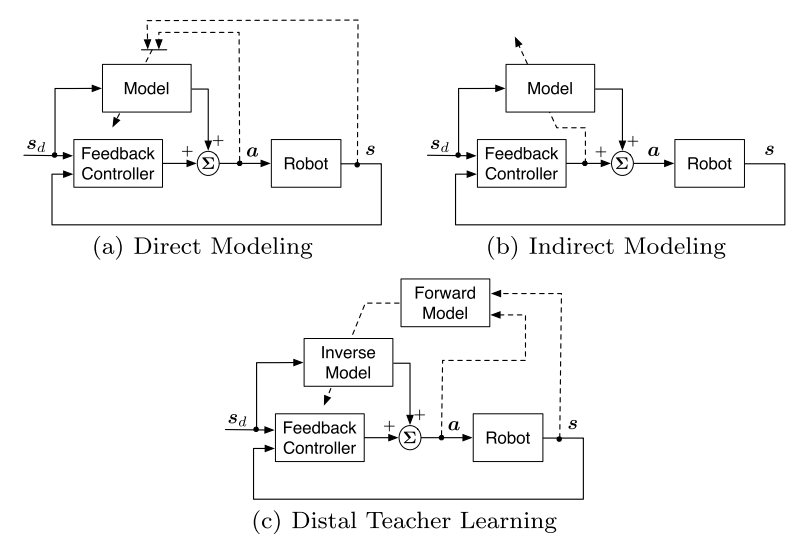
\includegraphics[scale=0.4]{Imatges/arquitectures-d'aprenentatge.png}
\caption{Esquema de cada arquitectura d'aprenentatge \cite{Nguyen-Tuong2011}}
\end{center}
\end{figure}


\paragraph{}Un dels beneficis de tenir el model d'un robot és poder fer simulacions virtuals del robot, de tal manera que no es provoca cap desgast al robot real, ni es poden donar situacions de perill. Tot i ser de gran utilitat, els simuladors també tenen les seves limitacions, és difícil simular la física d'un robot (actuadors, interaccions amb l'entorn, sensors\dots) de manera realista, a més, passar de simulacions a un robot real no sempre és fàcil \cite{Hohl2006}.

\paragraph{}Ara bé, existeixen una gran multitud de simuladors cada un amb les seves peculiaritats. Alguns dels que s'ha pogut extreure informació i que podrien ser de més interès són els següents:

\begin{description}
\item[Webots\texttrademark] \cite{Michel2004} Simulador de robots mòbils desenvolupat per Cyberbotics Ltd. La física està basada en Open Dinamic Engine (\textit{ODE}), per així simular una dinàmica més acurada. Aquest \texttt{software} proveeix un entorn de treball per modelar i programar el teu propi robot, a més inclou models de diversos robots com són Sony Aibo, Khepera, Lego Mindstorms\texttrademark o Pioneer2.

\item[SimRobot] \cite{Laue2006a} Aquest és un simulador genèric de robots en 3D. Com el Webots\texttrademark , el SimRobot també es basa en la física d'\textit{ODE}. Un dels inconvenients d'aquest simulador és que no es possible transferir els controladors de la simulació al robot real.

\item[Gazebo] \cite{Khatib2002} És un simulador multi-robots en 3D. Aquest, al igual que Webots\texttrademark , permet el modelatge del teu propi robot, tot i ser en llenguatge C, també es diferencia amb Gazebo pels models que inclou, que són el Pioneer2DX i el SegwayRMP.
\end{description}

\paragraph{}Com s'ha mencionat, en les descripcions anteriors, Webots\texttrademark inclou un model del Sony Aibo, dissenyat en \cite{Hohl2006}. Aquest té implementat l'estructura cinemàtica, propietats dinàmiques\footnote{Masses i moments d'inèrcia}, el seu control i l'aspecte gràfic. Per altre banda, també es pot simular els sensors de distància i els de les potes. El model té certes limitacions, els sensors del llom, cap, acceleròmetres i tèrmics no estan implementats per poder ser simulats. 

%Diferents simuladors que hi ha i com treballen

%"We developed a model of the Aibo robot. This involved implementing its graphical aspect, replicating its kinematic structure, its dynamics properties (masses and moments of inertia) and its control."

%"Aibo’s Position Sensing Device (PSD) is modeled by a DistanceSensor node of “infra-red” type (see Fig. 3). We modeled Aibo’s paw touch sensors by TouchSensor nodes which return binary values. Because only the paw touch sensors are of interest for the simulation of Aibo’s movements, the back sensors, the chin switch and the head sensors are not yet included in the model. Acceleration and thermo sensors do not have corresponding Webots nodes and can therefore not be simulated. Similarly, the speaker and microphone cannot be simulated in Webots, but there is a Camera node type, which we used to include Aibo’s color camera in the model."

%Model del robot--> Durant molt temps el metode d'utilitzacio dels robots ha estat creant models d'ells i a partir d'aquest fer els estudis pertinents.
%Que és un model? Quina informació t'aporta? Com es pot fer un model d'un robot(a mà, automàticament)? Quins inconvenients et pot portar el fer un model? De que serveix tenir un model?(saber com t'afecta una perturbacio i fer les accions tals que contraresten)Ara bé, si nomes utilitzes el model sense cap altre mètode després has de picar el codi de totes les possibilitats

\subsubsection*{(3) Aprenentatge supervisat}
\addcontentsline{toc}{subsubsection}{Aprenentatge supervisat}

\paragraph{}En l'aprenentatge supervisat, un agent extern presenta una sèrie de dades d'exemple, prediccions correctes a fer en diferents situacions \cite{Kober2009}. A partir d'aquestes dades d'entrenament, s'ha d'extreure un model per tal que, en una situació desconeguda, s'esculli l'acció correcte. L'aprenentatge supervisat és, segons \cite{Cord2008}, la metodologia més important d'aprenentatge automàtic i amb molt pes en el processament de dades multimèdia.

\paragraph{}Les dades a estimar poden ser binaries,on s'escull si una dada desconeguda és d'un tipus (p. e. pertany a un grup o no), o numèriques, on s'utilitza la regressió per aproximar. Tant siguin unes o altres, les bases de l'aprenentatge supervisat són: (1) el model, (2) la funció de pèrdua i la d'error d'aproximació, i (3) procediment d'optimització \cite{Alpaydin2004}.

\begin{enumerate}

\item El model es representa com $g(x|\theta)$\footnote{La x són les entrades, mentre $\theta$ són els paràmetres}, on \textit{g}(·) és la classe d'hipòtesi i els valors de $\theta$ donen una hipòtesi en concret d'entre les possibles en el model.

\item La funció de pèrdua, \textit{L}(·), quantifica la diferència entre la sortida desitjada, $r^t$, i l'aproximació $g(x^t|\theta)$, mentre la suma de les pèrdues de cada cas és l'error d'aproximació \begin{equation} \label{eq:er-aprox}
E(\theta|X)=\sum_{t} L(r^t,g(x^t|\theta))
\end{equation}

\item El procediment d'optimització per trobar $\theta^*$ que minimitza l'error total és:
\begin{equation} \label{eq:theta-opt}
\theta^*=arg\,\operatorname*{min}_\theta E(\theta|X)
\end{equation}
En models complexes, seria més convenient utilitzar mètodes basats en el gradient (p. e. gradient descendent, gradient conjugat, gradient biconjugat\dots) o l'algorisme de recuita simulada\footnote{A partir d'una solució inicial es selecciona una nova, aleatòriament, pròxima a la inicial. Si es millor s'hi queda, i sinó, segons una certa probabilitat, torna a l'anterior o es queda en la nova. Això es repeteix fins a la condició d'acabament\cite{Torrent-Fontbona2013}}.

\end{enumerate}

\paragraph{}Un dels algorismes més simples és la classificació per veí més proper, aquest és molt útil per entendre el funcionament bàsic de l'aprenentatge supervisat \cite{Learned-Miller2014}. En aquest cas, les dades d'entrenament estan etiquetades, per tant, cada una pertany a un grup en concret. Suposem que es té alguna forma de fer el càlcul de la distància entre dues mostres $x_{1}$ i $x_{2}$, expressat com $D(x_{1}, x_{2})$.

\paragraph{}Llavors amb la forma simplificada, pel cas de binàries, de \eqref{eq:theta-opt}
\begin{equation} \label{eq:theta-opt-exemple}
i^*=\operatorname*{arg\,min}_{i\in\{1\dots n\}} D(x_{t}, x_{i})
\end{equation}
Sent $x_{t}$ la dada a classificar i $x_{i}$ l'exemple més pròxim. Després de trobar $i^*$, s'assigna l'etiqueta de $x_{i}$ a $x_{t}$, queda així classificada la dada. Per suposat, aquesta assignació és una suposició, pot ser correcte o incorrecte.


\subsubsection*{(4) Aprenentatge per reforç}
\addcontentsline{toc}{subsubsection}{Aprenentatge per reforç}

\paragraph{}En la robòtica, l'aprenentatge per reforç proveeix d'unes eines molt útils per tal de crear comportaments sofisticats i amb gran dificultat de disseny. Permet a un robot desenvolupar el seu propi comportament a base de prova i error. En aquest cas, el dissenyador, en lloc de donar unes dades per explícitament crear la solució al problema, tan sols proveeix una realimentació amb una funció objectiu de valors escalars que mesura la bondat de l'acció anterior. Per tant, un agent explora les possibles estratègies i després rep una recompensa per l'acció feta, intentant sempre maximitzar la recompensa acumulada durant el seu temps de vida \cite{Kober2009}.

\paragraph{}Aquest agent i el seu entorn pot ser modelat com un estat \textit{s}$\in$\textit{S}\footnote{Un estat \textit{s} conté la informació necessaria per descriure la situació actual i futures.} i una acció \textit{a}$\in$\textit{A}\footnote{Un estat del sistema es controlat o carregat per una acció \textit{a}.}. Una recompensa es donada a l'agent, per cadascuna de les accions que desenvolupa, en funció de l'estat i les observacions. L'objectiu de \texttt{RL} és crear una política\footnote{Per política s'entén com en \cite{iec-dlc} "\textit{Manera de conduir un afer.}"} $\pi$ que maximitza la recompensa acumulada escollint unes accions \textit{a} en determinats estats \textit{s}.

\paragraph{}La idea clàssica d'aprenentatge per reforç es prenia des del punt de vista que l'agent consistia en un procés de decisions de Markov (\textit{Markov Decsion Process} o \textit{MDP})\footnote{Conjunt d'estats \textit{S}, accions \textit{A}, recompenses \textit{R} i probabilitats de transició T, aquest últim defineix la dinàmica del sistema per predir l'efecte de l'acció en un estat donat.} on la propietat de Markov estableix que el següent estat \textit{s}$'$ i la recompensa estan definits tan sols per l'acció \textit{a} i l'estat \textit{s} \cite{Sutton1998}. %Actualment, no tots els estudis que es fan segueixen el concepte de \textit{MDP}, ja que s'utilitza el \texttt{RL} sense tenir definit el sistema dinàmic, per tant, sense saber l'efecte de l'acció sobre l'estat. 

%S'hauria de posar la parta comentada anteriorment? Tot i que del sistema dinamic només se'n parla en el peu de pagina?

\paragraph{}L'acumulació de recompensa és el que es maximitza, per tant segons el mètode d'atorgar-la definirà el comportament òptim \cite{Kober2009}. Existeixen diversos models, aquí se n'exposen tres:
\begin{description}


\item[Horitzó finit] Aplicat en models on es sap en quants passos es resol el problema, maximitza la recompensa per \textit{H} passos.
\begin{equation}
J=E\left\{ \sum_{h=0}^{H} R_{h} \right\}.
\end{equation}

\item[Model de descompte] Un factor de descompte ($\gamma\in[0,1)$) a la recompensa futura. Aquest és introduït manualment i determina en quina proporció afecta el futur.
\begin{equation}
J=E\left\{ \sum_{h=0}^{\infty} \gamma^h R_{h} \right\}.
\end{equation}

\item[Recompensa mitja] Finalment en aquest es té en compte la mitja total de les recompenses. El problema d'aquesta és que no es pot diferenciar si s'esta afavorint l'inici o el final del temps de vida.
\begin{equation}
J=\lim_{H \to \infty} E\left\{ \frac{1}{H}\sum_{h=0}^{H} R_{h} \right\}.
\end{equation} 

\end{description}


\subsubsection*{(5) Algorismes avançats}
\addcontentsline{toc}{subsubsection}{Algorismes avançats}

\begin{description}

\item[CPG] \textit{Central Pattern Generators}, la idea és crear una arquitectura capaç de generar coordinació entre diferents elements, independentment de la tasca a realitzar i de la plataforma robòtica utilitzada. Una forma de veure-ho és des del punt de vista dels autors de \cite{Tellez2005a}:
\begin{quotation}
"\textit{\dots we see the robot’s mind as a group of different modules each one in charge of its own device (sensor or actuator) that interacts with the rest of modules\dots} "
\end{quotation}

\paragraph{}Aquesta cita podria ser traduïda com que cada dispositiu encarregant-se d'ell mateix, però amb la interacció amb els altres, tots junt arriben a crear la ment del robot.

\paragraph{}Per poder dur a terme aquesta arquitectura es requereixen de dos tipus d'algorismes: (1) algorismes neuro-evolutius, per poder cooperar entre mòduls i controlar els elements associats; i (2) algorismes co-evolutius, per instruir i arribar a un objectiu comú entre tots.

%Necessari posar antecedents?? (\cite{Tellez2005a})
%using neural oscillators and Central Pattern Generators (CPG) [3][4][5][6], like for example the use of CPGs for the control of several postures and movements [7]

\item[CBR] \textit{Case Based Reasoning}, aquest algorisme podria ser considerat de la família de l'aprenentatge supervisat. Consisteix l'aproximació de l'acció correcte a través de dos tipus de dades: (1) dades d'entrenament, del mateix estil que les del supervisat; i (2) extretes a partir de la pròpia experiència. El cicle de funcionament del CBR seria el següent: (i) prendre el cas o els casos més semblants a la situació actual, dels que estan emmagatzemats; (ii) adaptar el cas pres a la situació; (iii) avaluar com de satisfactori ha estat la solució adoptada; (iv) aprendre d'aquest nou cas.

\item[GA] \textit{Genetic Algorithm}, és un mètode estocàstic de cerca que pren la idea de l'evolució biològica natural. Aquest pren uns antecedents aleatoris, d'aquests en treu solucions les quals s'hi provoca una mutació, per últim, les solucions alterades es converteixen en els antecedents. Aquest procés es repeteix fins arribar a la solució que s'adapta suficient a la funció objectiu o al limit de generacions.

\end{description}

%Aprenentatges, alguns no necessiten d'un model per poder treballar tot i que si es té un model poden desenvolupar les tasques amb més facilitat i precisió (si el model ha estat creat correctament)
%Aprenentatge supervisat i el no supervisat
%Aprenentatge per reforç (Q-learning, R-learning, DMP, etc)
%CPG i algorismes genètics


\label{Objectius}
\subsection*{Objectius}
\addcontentsline{toc}{subsection}{Objectius}

\paragraph{}L'objectiu principal del present TFG és l'optimització de l'adaptabilitat d'un robot quadrúpede, en aquest cas l'AIBO, a plans inclinats desconeguts pel robot. Per arribar a aquest objectiu s'han hagut de marcat uns objectius més concrets:
\begin{itemize}
\item Dissenyar un entorn de treball complert que permeti que l'algorisme utilitzat pugui ser processat en l'ordinador i enviar la informació necessària de forma remota a l'AIBO. En aquest cas l'entorn de treball tal que permeti això serà el ROS.
\item Utilització de l'algorisme més adequat, tenint en compte tant l'entorn del robot i ell mateix, com l'abast del treball. Per això s'haurà de fer un estudi dels diferents mètodes existents que podrien ser útils per l'objecte del treball.
\item Dur a terme una fase d'aprenentatge pel robot. Per poder fer-ho, abans, s'haurà d'haver fet un estudi en profunditat del aprenentatge per reforç.
\item Realització de diferents proves per comprovar el correcte funcionament. Tant per poder comprovar, com per fer la fase d'aprenentatge del robot, és necessita d'una plataforma mòbil que en aquest cas ja està construïda, pel Carlos Ramos (estudiant de la EPSEVG)\cite{TFG_Carlos_Ramos}, però s'ha de millorar per fer-la més robusta.
\end{itemize},


\label{Abast}
\subsection*{Abast del treball}
\addcontentsline{toc}{subsection}{Abast del treball}

\label{Estructura}
\subsection*{Estructura del treball}
\addcontentsline{toc}{subsection}{Estructura del treball}

\newpage

\label{Estudis-preliminars}
\section{Estudis preliminars}

\label{AIBO}
\subsection{AIBO}
\paragraph{}L'AIBO (\textit{\texttt{A}rtificial \texttt{I}nteligence Ro\texttt{BO}t}) és un robot quadrúpede dissenyat i fabricat per Sony Corporation, amb aparença canina. El primer model que va ser tret al mercat fou el \textit{ERS-110} el 1999, a partir d'aquest, i després de tres generacions, el 2003 s'arribà al \textit{ERS-7}, molt més sofisticat que els predecessors, tot i que en el 2006 s'aturà la producció de la família AIBO. El \textit{ERS-7} és el model que s'estudia i s'utilitza en el present treball.

\paragraph{}Aquest es considerat un robot autònom, per tant, és capaç d'extreure informació del seu entorn, funcionar per un període llarg sense la intervenció humana, moure alguna o totes les parts d'ell mateix dins d'un entorn de treball sense l'ajut d'un humà i, finalment, evitar situacions de perill per les persones, els bens o ell mateix, si no és per especificacions del propi disseny.

\paragraph{}L'aplicació d'aquest robot autònom està enfocada en ser utilitzat en propòsits d'entreteniment, tot i ser, en molts casos, utilitzat en tasques d'investigació. Els robots autònoms corrents solen ser dissenyats per desenvolupar tasques de seguretat o treballs perillosos, ara bé, en aquests casos no es pot tolerar cap tipus d'error en les operacions crítiques. Mentre els que estan dissenyats per usos d'entreteniment, en el cas que es produís algun error no seria un amenaça per la vida \cite{Fujita2000}.

\paragraph{}Els dissenyadors de l'AIBO han perseguit l'objectiu d'aconseguir que el comportament sigui el màxim de real possible, que sembli viu. Per assolir-ho, han avançat per diferents camins:
\begin{itemize}
\item Estímuls
\begin{itemize}
\item Comportaments reflexius i deliberats segons una escala de temps.
\item Comportaments per ordres externes i per desigs interns (instints i emocions).
\item Motivacions independents donades per parts del robot com coll, cua i potes.
\end{itemize}
\item Instints i emocions amb els que pot canviar el comportament davant d'altres estímuls externs.
\item Aprenentatge i evolució, inicialment és com un nadó sense pràcticament cap coneixements. Així com passa el temps, l'AIBO aprèn i creix segons com el tractis. Per tant, podria arribar a comportar-se com un noi entremaliat, si no se li dona l'atenció necessària.
\end{itemize}

\label{Hardware}
\subsubsection{\textit{Hardware}}

\paragraph{}Les característiques del robot són les següents: \cite{Anshar2007}

\begin{itemize}
\item Processador MIPS R7000 de 576 MHz 
\item Memòria RAM de 64 MB
\item LAN sense fils, 802.11b (estàndard)
\item Targeta interna de memòria lectura/escriptura 
\item 18 articulacions PID, cadascuna amb un sensor de força
\begin{itemize}
\item 4 potes
\begin{itemize}
\item 3 articulacions cadascuna (elevació, rotació i genoll)
\item 1 sensor de pressió a cada peu
\end{itemize}
\item 3 articulacions al coll (moviment horitzontal, vertical i inclinació)
\item 2 articulacions a la cua (moviment vertical i inclinació)
\item 1 articulació a la boca
\end{itemize}
\item 2 orelles, on hi ha els micròfon estèreo i amb una articulació booleana (posició dalt o baix)
\item Altaveus de 500 mW
\item 26 LEDs independents
\item Càmera de vídeo
\begin{itemize}
\item Sensor d'imatge CMOS
\item 56.9$^{\circ}$ ample i 45.2$^{\circ}$
\item Resolucions: $208\times160, 104\times80, 52\times40$
\item 30 imatges per segon
\end{itemize}
\item 3 sensors de distància per infrarojos (un al cos i dos al nas, d'aquests dos, un és per objectes llunyans i un altre per pròxims)
\item Acceleròmetres \textit{X}, \textit{Y} i \textit{Z}
\item 4 botons sensorials de pressió (un al cap i tres al llom)
\item 1 botó booleà sota la boca
\item Sensor de vibració
\item Actualització dels sensors cada 32 ms, amb 4 mostres per actualització
\item Dimensions: $319\times180\times278$
\item Pes aproximat: 1,65 kg (bateria i targeta de memòria incloses)

\end{itemize}

\begin{figure}[H]
	\centering
        \begin{subfigure}[h]{0.5\textwidth}
                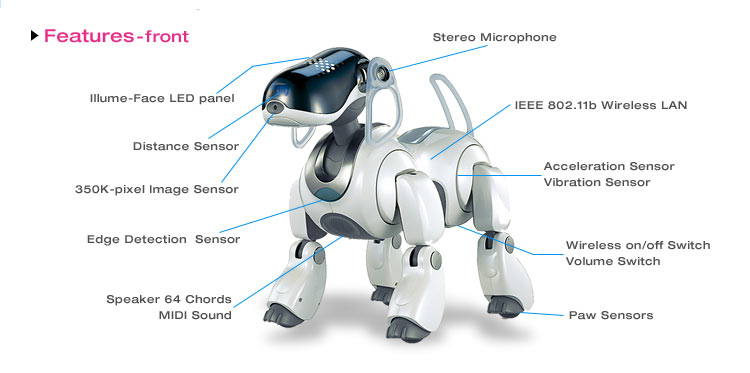
\includegraphics[width=\textwidth]{Imatges/ERS-7(front)}
                \caption{(vista frontal)}
        \end{subfigure}%
        \begin{subfigure}[h]{0.5\textwidth}
                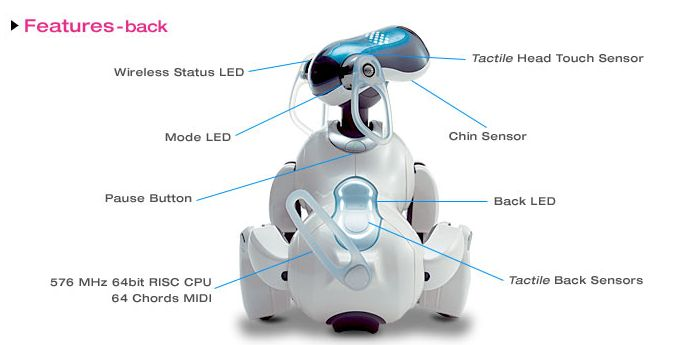
\includegraphics[width=\textwidth]{Imatges/ERS-7(back)}
                \caption{(vista posterior)}
        \end{subfigure}
        \begin{subfigure}[bl]{0.5\textwidth}
        			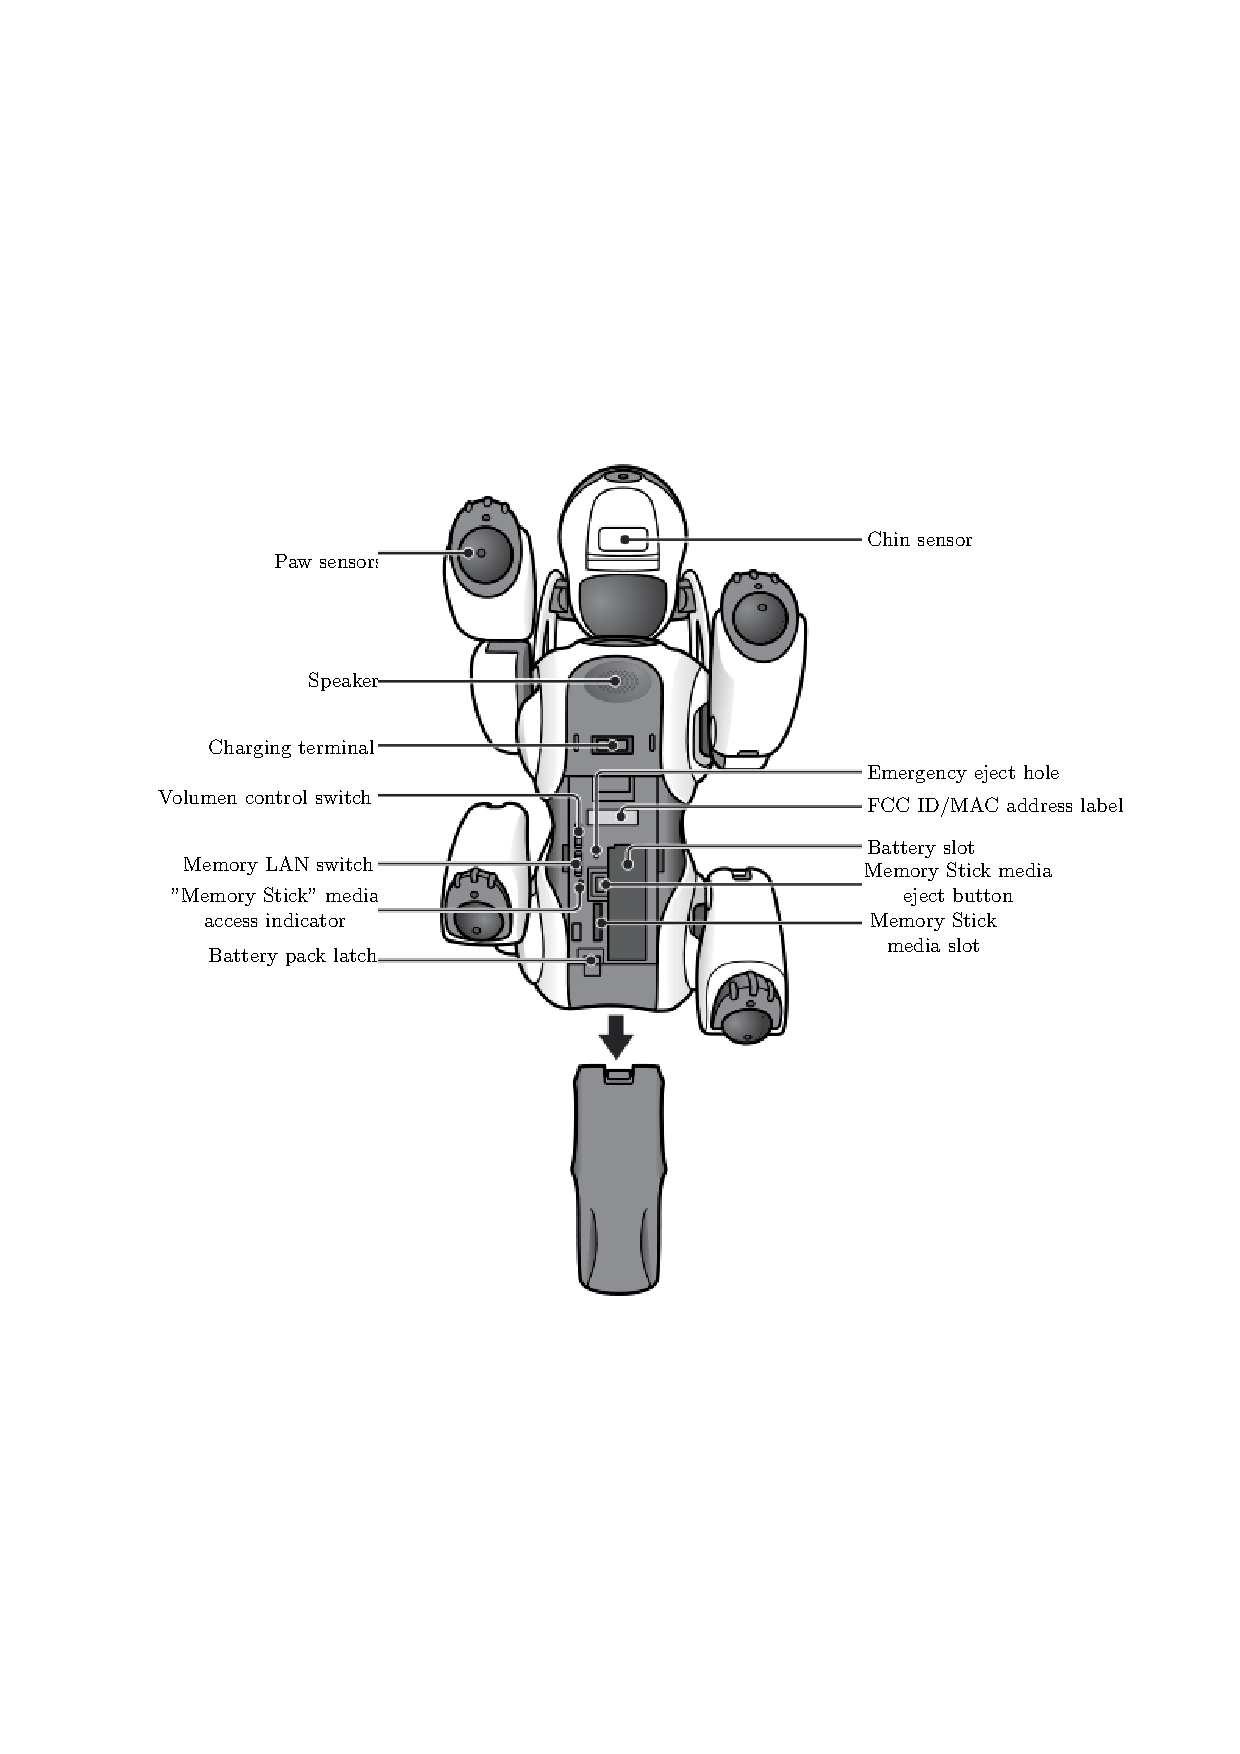
\includegraphics[width=\textwidth]{Imatges/ERS-7(stomach)}
                \caption{(vista inferior)}
        \end{subfigure}
        \caption{AIBO ERS-7 \cite{Aibo_Images}}
\end{figure}

\paragraph{}Les articulacions PID, segons la seva funció i les pròpies limitacions físiques tenen uns rangs de treball diferents, aquest són els que s'exposen tot seguit: 

\begin{table}[H]
\begin{center}
\begin{tabular}{| c | c | c | c |}
\hline
Name & Range & Units & Description\\ \hline \hline
legRF1    &    range=[-134.000000,120.000000]  & unit=deg & Right fore legJ1\\
legRF2    &    range=[-9.000000,91.000000]     & unit=deg & Right fore legJ2\\
legRF3    &    range=[-29.000000,119.000000]   & unit=deg & Right fore legJ3\\
legRH1    &    range=[-134.000000,120.000000]  & unit=deg & Right hind legJ1\\
legRH2    &    range=[-9.000000,91.000000]     & unit=deg & Right hind legJ2\\
legRH3    &    range=[-29.000000,119.000000]   & unit=deg & Right hind legJ3\\
legLF1    &    range=[-120.000000,134.000000]  & unit=deg & Left fore legJ1\\
legLF2    &    range=[-9.000000,91.000000]     & unit=deg & Left fore legJ2\\
legLF3    &    range=[-29.000000,119.000000]   & unit=deg & Left fore legJ3\\
legLH1    &    range=[-120.000000,134.000000]  & unit=deg & Left hind legJ1\\
legLH2    &    range=[-9.000000,91.000000]     & unit=deg & Left hind legJ2\\
legLH3    &    range=[-29.000000,119.000000]   & unit=deg & Left hind legJ3\\
neck      &    range=[-79.000000,2.000000]     & unit=deg & Neck tilt1\\
headTilt  &    range=[-16.000000,44.000000]    & unit=deg & Neck tilt2\\
headPan   &    range=[-91.000000,91.000000]    & unit=deg & Head pan\\
tailPan   &    range=[-59.000000,59.000000]    & unit=deg & Tail pan\\
tailTilt  &    range=[2.000000,63.000000]      & unit=deg & Tail tilt\\
mouth     &    range=[-58.000000,-3.000000]    & unit=deg & Mouth\\
\hline
\end{tabular}
\end{center}
\caption{Rangs de funcionament de les articulacions \cite{Urbi_Docs}}
\end{table}

%Alguna solució per posar la taula al seu lloc
%\pagebreak funciona, però la pagina anterior amb queda amb un espai interlinial molt gran
%El mateix passa amb el parametre [H]


\label{Software}
\subsubsection{\textit{Software}}
%\paragraph{}Com s'ha esmentat anteriorment, l'AIBO aprèn i evoluciona segons el seu entorn amb uns coneixements inicials quasi nuls. Però sí que incorpora unes funcions bàsiques, com ara, caminar, reconeixement de veu, reproducció de sons, entre moltes altres.


%\paragraph{}Actualment, l'AIBO per defecte té multitud facultats, com ara, caminar en diferents direccions sense perdre l'equilibri o quedar-se en una posició de repòs estable, entre d'altres. Tot i que això només és possible en condicions òptimes (terreny pla i llis, sense forces externes que actuïn sobre el robot, etc.). Aquestes funcions i més ja han estat desenvolupades en llenguatges com OPEN-R o Tekkotsu (nivell mitjà) o Urbi (nivell alt). El repte és poder aconseguir fer això i més en ROS (\textit{Robot Operating System}), que proveeix un entorn de treball òptim per la creació de programari per a qualsevol robot, i per tant pot ser exportable de l'AIBO a qualsevol altre robot que compleixi els requisits mínims de \textit{hardware}.  
  


\subsection{ROS}
\label{ROS}
\paragraph{}\textit{\texttt{R}obot \texttt{O}perating \texttt{S}ystem} \cite{ROS} és un entorn de treball \texttt{open-source} i flexible per la programació de robots. Les bases d'aquest projecte s'iniciaren en unes investigacions a Stanford el 2007, on es varen dur a terme diferents prototips d'entorns de treball per programari de robots, com ara STanford Artificial Intelligence Robot (\textit{STAI}) o Personal Robotics (\textit{PR}). Més endavant, \textit{Willow Garage}, una empresa inversora en robòtica, va proveir recursos per tal de millorar el concepte i permetre crear implementacions correctament testejades. Finalment, amb la col·laboració desinteressada de incomptables investigadors, millorant el nucli de ROS i les eines principals que proveeix, s'ha arribat al que és ara, una plataforma àmpliament utilitzada en les investigacions de robòtica.

\paragraph{}En el moment de la redacció d'aquest treball, la versió més actual de ROS és la \textit{ROS Hydro Medusa}, publicada el setembre de 2013, i pròximament es publicarà la \textit{ROS Indigo Igloo}. La Hydro està dissenyada especialment per Ubuntu 12.04 LTS (\textit{Precise}), tot i suportà també altres sistemes Linux, Mac OS X, Android i Windows en altres graus.


\subsubsection{Estructura de ROS}
\paragraph{}ROS ofereix una interfície que permet la comunicació entre processos per tal de processar dades conjuntament, és comú referir-s'hi com a capa intermèdia. Els conceptes fonamentals de la implementació de ROS són els \texttt{nodes}, \texttt{Master}, \texttt{messages}, \texttt{services}, \texttt{topics} i \texttt{bags}.

\begin{itemize}
\item \textbf{Nodes}: Els \texttt{nodes} són processos que realitzen càlculs. Típicament, un sistema compren multitud de \texttt{nodes}. En aquests casos és útil entendre les comunicacions entre \texttt{nodes} com un graf, amb arcs que uneixen els que s'estan comunicant.

\item \textbf{Master}: El ROS \texttt{Master} proveeix els noms d'enregistrament dels \texttt{nodes}, \texttt{topics} i \texttt{services} existents als altres \texttt{nodes}. Per tant, el \texttt{Master} rep la informació de registre dels \texttt{nodes} i després aquest informa als altres \texttt{nodes} per tal que puguin establir, entre ells, connexions de forma adequada. 

\item \textbf{Messages}: Els \texttt{nodes} es comuniquen un amb l'altre mitjançant \texttt{messages}. Aquest són simplement estructures de dades, que poden anar des d'\texttt{integrer}, \texttt{floats}, \texttt{booleans} fins a \texttt{arrays}.

\item \textbf{Topics}: Un \texttt{node} envia un \texttt{message} mitjançant la publicació d'aquest en un \texttt{topic} donat. El \texttt{topic} és el nom que s'utilitza per identificar el contingut d'un \texttt{message} concret. 

\item \textbf{Services}: El \texttt{service} és el nom que ha d'utilitzar un \texttt{node} per enviar un \texttt{message}, amb la funció de sol·licitar una resposta que depèn del \texttt{message} enviat.

\item \textbf{Bags}: Els \texttt{bags} són un format per guardar i poder reproduir un altre cop les dades de \texttt{messages} de ROS. Aquests són de gran importància a l'hora de emmagatzemar dades i, per tant, per desenvolupar i testejar algorismes.
\end{itemize}

Aquesta capa intermèdia ofereix dos models de comunicació: (1) sistema de \textit{publicació/subscripció}; i (2) utilitzant \texttt{services}.
\begin{enumerate}
\item El sistema de \textit{publicació/subscripció} és anònim, asíncron i les dades poden ser capturades i rellegides sense canvis en el codi. Per tant, si per fer una certa tasca es requereix de les dades d'una altre tasca, com per exemple un sensor, llavors a partir de subscriure's al \texttt{topic} corresponent es poden llegir les dades que publica la tasca (sensor). Pot haver-hi múltiples publicadors i subscriptors per un únic \texttt{topic} i, en general, entre ells no saben de l'existència dels altres.

\item Els \texttt{services} estan definits per dos \texttt{messages}, un és la demanda que ha fet el \texttt{node} i l'altre és la resposta a aquesta demanda. Per tant, el seu ús és molt simple, en el moment que es crida un \texttt{service}, amb les dades que aquest requereixi, el procés dona una resposta al \texttt{node} segons les dades que s'han enviat.
\end{enumerate}

\subsubsection{Objectius de ROS}

\paragraph{}El principal objectiu de ROS és poder \textit{reutilitzar} el codi de desenvolupament i d'investigacions en robòtica. L'estructura de processos distribuïts permet aquest fet, ja que pot executar-se un procés (amb un codi determinat) de forma individual i acoblar-se fàcilment al conjunt. A més, aquests processos poden agrupar-se en \texttt{Packages} i \texttt{Stacks} i ser compartits de forma senzilla.

\paragraph{}D'altra banda, també és tenen unes altres finalitats \cite{Quigley}: (1) descentralització; (2) plurilingüisme; (3) estar basat en eines; (4) ser una capa intermèdia fina; (5) gratuïta i \texttt{open-source}.

\begin{enumerate}

\item Descentralització\\
ROS està estructurat de forma que els processos estan distribuïts, amb la possibilitat de trobar-se en \texttt{hosts} diferents, però funcionant conjuntament. Altres entorns de treball, que poden també treballar amb múltiples processos i \texttt{hosts}, si es basen en un servidor central, podrien tenir problemes en una xarxa heterogènia\footnote{Una xarxa heterogènia és una xarxa de connexió d'ordinadors i altres dispositius amb diferents sistemes operatius i/o protocols.\cite{Delphinanto2011}}.

\item Plurilingüisme\\
Cada programador és un món, cadascú té el seu llenguatge de programació preferit, sigui per la raó que sigui. Per això, ROS s'ha dissenyat per ser un llenguatge neutral. Actualment, ROS admet quatre llenguatges de programació: (1) \textit{C++}, (2) \textit{Python}, (3) \textit{Octave} i (4) \textit{LISP}, havent altres en desenvolupament.

\item Basat en eines\\
S'ha optat per dissenyar un nucli simple, on s'utilitzen multitud d'eines per construir i fer funcionar els diversos components de ROS, en vers, de dissenyar un enorme entorn de treball, tot en un. Tot i haver-se implementat alguns serveis en el propi nucli, s'ha intentat distribuir tot en mòduls separats. La pèrdua d'eficiència compensa els guanys en estabilitat i complexitat del conjunt.

\item Capa intermèdia fina\\
En molts casos, és molts difícil \textit{"extreure"} la funcionalitat d'un codi, del seu context original, per a poder ser reutilitzat, això és degut a factors provocats pel propi entorn de treball d'origen. Per això, en ROS s'indueix a la independència dels algorismes, amb el nucli del ROS, creant-los en llibreries separades. Es facilita l'extracció de codi i la seva reutilització a traves d'aquest fet, entre d'altres característiques de la interfície.

\item Gratuït i \texttt{open-source}\\
El codi natiu de ROS està disponible públicament. Aquest és un fet que permet facilitar el testeig i correcció de \texttt{software} en tots els nivells. 

\end{enumerate}


\subsubsection{Eines de ROS}
\paragraph{}Com s'ha comentat breument en l'apartat anterior, ROS és basa, en gran part, en la multitud d'eines que disposa. Aquestes eines poden arribar a dur a terme varies tasques diferents, per exemple, navegar per l'arbre de codi font, obtenir i establir els paràmetres de configuració, visualitzar les connexions entre processos, mesurar la utilització d'ample de banda, exposar de forma gràfica les dades dels \texttt{message}, i més. A continuació es comenten breument alguns dels més utilitzats:
\begin{itemize}
\item \texttt{rviz}\\
Rviz és un entorn de visualització 3D que pot combinar les dades dels sensors del robot i el model que és té, juntament amb altres dades 3D que se li aporti, per poder visualitzar el conjunt.

\item \texttt{rosbag} i \texttt{rxbag}\\
Rosbag és la comanda que et permet emmagatzemar i reproduir de nou les dades d'un \texttt{message} en un arxiu \texttt{bag}. Per altre banda, rxbag és un visualitzador per a les dades emmagatzemades dins els arxius \texttt{bag}.

\item \texttt{rxplot}\\
Rxplot permet veure dades escalars publicades en els \texttt{topics} de ROS.

\item \texttt{rxgraph}\\
Rxgraph exposa visualment amb un gràfic com funcionen els processos de ROS i les seves connexions, en aquell instant.

\end{itemize}

%Afegir apartat de packages i messages d'interés (per tal d'explicar el actionlib, dmp, sensor_msgs.msg (JointState), control_msgs.msg (FollowJointTrajectoryGoal, FollowJointTrajectoryAction), trajectory_msgs.msg (JointTrajectoryPoint) i altre que es puguin trobar)
%http://docs.ros.org/api/sensor_msgs/html/msg/JointState.html
%http://docs.ros.org/api/control_msgs/html/action/FollowJointTrajectory.html
%http://docs.ros.org/api/trajectory_msgs/html/msg/JointTrajectoryPoint.html

%Fins ara no s'ha donat suport oficial a AIBO en ROS...
%topics que té l'AIBO actualment
%Ricardo Téllez
\label{Estabilitat}
\subsection{Estabilitat}
%Com definirem estabilitat, diferents mètodes...

\label{Algorismes}
\subsection{Algorismes de resposta davant pertorbacions}

\paragraph{}En la robòtica, com en qualsevol àmbit, per un mateix problema poden ser utilitzades infinitat de solucions. Ara bé, el tret característic de l'enginyeria és que d'entre la multitud de possibilitats, s'esculli la més òptima segons les condicions del moment. Abans d'optar per una opció, s'ha de tenir una idea clara del que aporta cadascuna i observar com s'adapta a la problemàtica actual.

\paragraph{}En l'estat de l'art, s'han esmentat algunes de les possibilitats per dur a terme els objectius fixats inicialment. Aquestes opcions han estat explicades anteriorment, amb una breu descripció i trets característics que podrien ser d'interès pel nostre cas. A continuació, s'exposa com cadascuna podria adaptar-se al problema, mencionant els seus avantatges i inconvenients. Al final, s'escull la més adient pel cas i se'n fa una descripció més acurada. 

\subsubsection{Model del robot}

%"the execution of robot programs inside a simulator offers the possibility of directly debugging and testing them. This is a great benefit when working with platforms that do not offer any direct debugging facilities"

%"Simulators, of course, do have limitations and there are some problems to be solved. It is difficult to simulate the physics of a robot (actuators, interaction with the environment, sensors) realistically, and the transfer from simulation to the real robot is not always simple."

%Creació d'un model i fer estudi d'aquest model per saber davant una pertorbació com ha de ser les entrades dels actuadors per tal de estar en una posició d'estabilitat

%Supervised learning, a partir de moltes mostres d'indicacions i com ha de d'actuar per estar estable, pren una funció que aplicarà en els casos futurs.
%Noise: (1) Pot haver-hi impresicions en la gravacio de atributs d'entrada (2) Pot haver-hi errors en el "labeling" dels punts de datos (3) Poden existir atributs adicionals que no s'han tingut en compte i que afecten al "labeling", aquests poden ser "hidden or latent" i pot ser que no siguin observables

%Reinforcement learning, Q-learning i DMP (learning by demostration)

%Affordance: Mes o menys es podria entendre com els sensors i actuaduadors serien moduls neuronals que envien informació ja filtrada als altres moduls neuronals de tal manera que vagi enfocat a fer una tasca determinada

\newpage
\section*{Agraïments}
\addcontentsline{toc}{section}{Agraïments}

\newpage

\label{Referencies}
\addcontentsline{toc}{section}{Referències}
\bibliography{./Bibliografia/library}



\appendix
\clearpage % o \cleardoublepage
\addappheadtotoc
\appendixpage

\section{Instal·lació de ROS, llibreries d'Urbi i paquet aibo server}

\paragraph{}Tot seguit es mostren els passos a seguir per tal d'instal·lar ROS i com afegir una carpeta al la variable \texttt{ROS$\_$PACKAGE$\_$PATH}\footnote{Aquí es troben les direccions de les carpetes on ROS cerca els \texttt{packages}.}.

\begin{enumerate}

\item Preparar per instal·lar ROS (en aquest cas per Ubuntu 12.04 32 bits).\\
\texttt{sudo sh -c 'echo "deb http://packages.ros.org/ros/ubuntu precise main" \\ > /etc/apt/sources.list.d/ros-latest.list'}

\item Configurar claus de ROS.\\
\texttt{wget http://packages.ros.org/ros.key -O - | sudo apt-key add -}

\item Instal·lar ROS-fuerte.\\
\texttt{sudo apt-get update}\\
\texttt{sudo apt-get install ros-fuerte-desktop-full}

\item Per tal que els \texttt{packages} en la carpeta del propi ROS puguin ser trobats més còmodament. La comanda final és per poder seguir treballant en el mateix terminal.\\
\texttt{echo "source /opt/ros/fuerte/setup.bash" $\gg$ $\sim$/.bashrc.\\
source $\sim$/.bashrc}

\item Es necessiten instal·lar alguns paquets per poder continuar, com és el \texttt{rosws}, que es part del paquet \texttt{rosinstall}.\\
\texttt{sudo apt-get install python-rosinstall python-rosdep}

\item Es crea una carpeta de treball, extensió de la propia de ROS.\\
\texttt{rosws init $\sim$/fuerte /opt/ros/fuerte}\\
\texttt{mkdir $\sim$/fuerte/sandbox}\\
\texttt{rosws set ~/fuerte/sandbox}

\item Per acabar la instal·lació de ROS, es repeteix l'acció (4), però en aquest cas, per poder ser trobats els \texttt{packages} de la carpeta que s'ha creat.\\
\texttt{echo "source $\sim$/fuerte/setup.bash" $\gg$ $\sim$/.bashrc\\
source $\sim$/.bashrc}

\item Tot seguit, s'ha d'instal·lar la llibreria d'urbi. En aquest cas, tan sols s'ha descarregar l'arxiu comprimit\footnote{\url{http://www.gostai.com/downloads/urbi/1.5/urbi-sdk-1.5-l0258c7a-i486-linux-gnu-gcc-4.1.tar.gz}} i extreure'l en \textbackslash .\\

\item Finalment per instal·lar el paquet d'Aibo server, s'ha de copiar la carpeta en alguna de les direccions de \texttt{ROS$\_$PACKAGE$\_$PATH} i compilar seguint aquest procediment:\\
\texttt{roscd aibo$\_$server/}\\
\texttt{rosmake --pre-clean}

\end{enumerate}

\section{Bibliografia}

\end{document}  

